%%%%%%%%%%%%%%%%%%%%%%%%%%%%%%%%%%%%%%%%%%%%%%%%%%%%%%%%%%%%%%%%%%%%%%%%
\chapter{Vergleich}
\label{sec:comparison}
%%%%%%%%%%%%%%%%%%%%%%%%%%%%%%%%%%%%%%%%%%%%%%%%%%%%%%%%%%%%%%%%%%%%%%%%
Es folgt nun eine Gegenüberstellung der einzelnen Frameworks, anhand der in Kapitel \ref{sec:methodik} definierten Kriterien. Als erster wird ein genereller Überblick über die einzelnen Fakten zu den Frameworks gegeben und deren Unterschiede beschrieben. Danach wird genauer auf relevanten Kriterien für das Revex Projekt eingegangen und ein persönliches Fazit zu den Frameworks gezogen.

\section{Gegenüberstellung der Frameworks}

{\large \textbf{Entwicklungskultur rund um die Frameworks}}\\\\
Alle Frameworks werden unter einer Open Source Lizenz zur Verfügung gestellt. Einige Lizenzen beinhalten aber ein Copyleft, was verlangt, dass die entwickelte Software ebenfalls wieder unter der gleichen Lizenz als \acrfull{OSS} zur Verfügung gestellt wird. Die wichtigste Copyleft-Lizenz ist die \acrfull{GPL}. Die GPL bestimmt, dass Software, welche eine Framework unter dieser Lizenz nutzt, wiederum nur unter GPL vertrieben werden darf. Die Apache License ist eine Lizenz ohne Copyleft, es ist daher zulässig Frameworks mit dieser Lizenz in proprietärer Software zu verwenden. Die \acrfull{CDDL} beinhaltet ein abgeschwächtes Copyleft, lizenzierter Code kann in einem anderen Framework verwendet werden, solange dieser Code nicht auf Dateiebene gemischt wird. Die CDDL verbietet nicht, entwickelte Software unter einer anderen Lizenz zu veröffentlichen. Für die reinen Nutzer von OSS, welche die Frameworks weder weiterentwickeln noch vertreiben wollen, spielen die Unterschiede der verschiedenen OSS-Lizenzen kaum eine Rolle. Will ein Entwickler jedoch seine Arbeitsergebnisse nicht als OSS veröffentlichen, darf er für seine Arbeiten keine OSS Frameworks verwenden, welche mit einem strengen Copyleft lizenziert sind \cite{openSource}. Die Lizenzen der einzelnen Frameworks könnten aus der Tabelle \ref{tableVergleich} entnommen werden.
\\\\
OSS wird durch Communities entwickelt, weiterentwickelt und gewartet. Dabei übernimmt die Community zahlreiche Aufgaben, die bei Closed Software vom Hersteller oder Anbieter wahrgenommen werden. In der Regel gibt es zu jeder OSS genau eine Community. User der Software können dabei ein registriertes Mitglied der Community sein und aktiv am Projekt als Entwickler oder Tester mitarbeiten. Die Qualität einer Software hängt dabei maßgeblich von der Aktivität und der Struktur der Community ab. Sind zahlreiche aktive Mitglieder mit unterschiedlichen Rollen am Projekt beteiligt, ist dies eine Grundlage für eine gute Qualität der Software \cite{openSource:community}. Alle untersuchten Frameworks weisen eine aktive und starke Community auf.
\\\\
Um die Anwendung neuer Frameworks zu lernen, lesen 78 Prozent der Entwickler die Dokumentation, 55 Prozent verwenden Codebeispiele und 29 Prozent fragen Kollegen \cite{robillard:apis}. Dadurch ist es besonders wichtig auf eine aktuelle Dokumentation des Source-Codes Zugriff zu haben. Wird nur eine veraltete Dokumentation zur Verfügung gestellt, kann es passieren das die entwickelte Software Sicherheitslücken hat oder mehr Zeit für eine korrekte Implementierung benötigt wird \cite{lethbridge:documentation}. Für alle Frameworks ist eine Dokumentation vorhanden. Die Dokumentation von Retrofit deckt dabei aber nur die grundlegende Funktionsweise ab und ist im Vergleich zu den anderen schwächer. Das Problem hierbei war, dass in der zweiten Jahreshälfte 2015 ein großes Update des Frameworks während des Evaluierungsprozesses durchgeführt wurde und die vorhandene Dokumentation dadurch teilweise veraltet war. Es konnten auch Codebeispiele für alle Frameworks gefunden werden, diese sind gut erklärt und ermöglichen es eine lauffähige Anwendung zu implementieren. Problematisch war es allerdings die gefunden Jersey Codebeispiele unter Android zu starten, da keines dieser speziell für Android entwickelt wurde. Es musste zuerst ein Workaround (siehe Kapitel \ref{workaroundAndroid}) durchgeführt werden, um die Beispiele auf einem Android Gerät starten zu können.
\\\\
{\large \textbf{Implementierung der REST-Frameworks}}\\\\
Einer der relevantesten Aspekte für den Evaluierungsprozess ist die Implementierung und Verwendungsweise der Frameworks. Bis auf Jersey sind alle Frameworks leicht einzubinden und zu benützen. Für Jersey muss zuerst ein Workaround durchgeführt werden, damit dieses Framework überhaupt unter Android genutzt werden kann. Die genaue Verwendungsweise der Frameworks wird in Kapitel \ref{chapter:frameworks} beschrieben.
\\\\
Es werden von allen Frameworks die gängigsten HTTP-Methoden unterstützt. Retrofit unterstützt dabei als einziges nicht die HTTP-Methode OPTIONS. Es ist auch möglich mit allen Frameworks den HTTP-Header zu erweitern bzw. zu verändern. Des weiteren ist es auch möglich alle möglichen Medientypen zu unterstützten, wenn ein Konverter dafür implementiert und beim Framework registriert wird. Endpoint URLs zum Server können dynamisch während der Laufzeit bei allen Frameworks verändert werden. 
\\\\
Wenn zeitraubende Aktionen ausgeführt werden sollen, wie z.B. das Herunterladen einer großen Datei aus dem Internet, langweilen sich User oft. Denn diese müssen dann warten bis der Request vollständig abgearbeitet wurde und können währenddessen nicht weiterarbeiten. Dies kann aber verhindert werden, indem zeitraubende Aktion im Hintergrund ausgeführt werden - in Form von asynchronen Requests \cite{louis:android}. Mithilfe aller Frameworks können asynchrone Requests modelliert werden. 
\\\\
Das HATEOAS Konzept wird von Jersey und Spring for Android unterstützt. Jedoch muss bei Spring for Android eine eigene Bibliothek \textquotedblleft Spring HATEOAS\textquotedblright\, eingebunden werden, damit eine Linkverfolgung möglich ist. Wenn das HATEOAS Konzept mit AndroidAnnotations verwendet werden soll, muss ebenfalls \textquotedblleft Spring HATEOAS\textquotedblright\, eingebunden werden und die Verwendung ist nur ohne Annotations möglich. Man greift dabei auf die Basis REST Implementierung zurück, welche Spring for Android ist. Retrofit unterstützt das HATEOAS Konzept nicht.
\\\\
Das registrieren von Error Handlern ist bei allen Frameworks möglich, dadurch können aussagekräftige Fehlermeldungen für den User erzeugt werden. Designrichtlinien für mögliche Geräte geben an, dass es sinnvoll ist, Rückmeldungen für Aktionen des Systems zu geben, wie beispielsweise eine Fehlermeldung, wenn der Server nicht erreichbar ist. Eine solche Rückmeldung sollte für den Benutzer verständlich sein. Zum Beispiel sind die Fehlermeldungen \textquotedblleft HTTP404 ERROR\textquotedblright\, und \textquotedblleft Diese Seite konnte nicht gefunden werden\textquotedblright\, äquivalent, die zweite Fehlermeldung ist aber für einen Großteil der User verständlicher \cite{gong2004guidelines}.
\\\\
{\large \textbf{Performance}}\\\\
Mobile Geräte haben längst Einzug in das Alltagsleben erhalten, viele Nutzer erweitern die Funktionalität der Geräte mit zahlreichen Anwendungen. Jede installierte App auf einen mobilen Endgerät hat Einfluss auf den Energieverbrauch. Je mehr Anwendungen auf eine Endgerät installiert sind und je öfter diese genutzt werden, desto höher ist der Energieverbrauch und die Betriebszeit sinkt dadurch massiv \cite{Wil2012}. Daher ist bei der Entwicklung darauf zu achten, dass der Energieverbrauch so gering wie möglich gehalten wird. Auswirkungen auf den Energieverbrauch eines Smartphones haben sowohl der Bildschirm, die \acrfull{CPU}, die Kommunikation über das Mobilfunknetz, als auch das WLAN-Modul. Werden die einzelnen Komponenten so wenig wie möglich beansprucht, ist der Energieverbrauch der Anwendung gering \cite{vetter}. 
\\\\
Umso länger und mehr Daten bei einem Request über das Mobilfunknetz oder das WLAN-Modul übertragen werden, desto mehr Energie wird verbraucht. Es sollte daher darauf geachtet werden, dass die Requestdauer möglichst gering ist und nicht unnötige Daten übertragen werden. Des weiteren ist die Rechenleistung von Smartphones  wesentlich geringer als jene von Notebooks. Daher ist bei der Entwicklung auch darauf zu achten, dass die CPU Beanspruchung der Apps gering gehalten wird, damit das System performant weiterarbeiten kann \cite{mittal:energy}. Außerdem sollte die benötigte CPU Leistung aus einem weiteren Grund möglichst gering sein, den die Hardware variiert von Smartphone zu Smartphone. Ist die benötigte CPU Leistung gering, ist es möglich die App auf nahezu allen mobilen Geräten zu installieren und zu starten \cite{joorabchi:challenges}. 
\\\\
Für den Performance Vergleich wurden daher sowohl die CPU-Auslastung, als auch die Dauer für GET- und POST Requests (Dauer der Netzwerkkommunikation) der einzelnen Frameworks gegenübergestellt. Um Vergleichswerte zu ermitteln, wurde jede App einzeln in einem Emulator gestartet und die gleiche Abfolge an Funktionsaufrufen durchgeführt. 
\\\\
Die Zeitdauer der GET-Requests bei der Abbildung \ref{getRequests} setzt sich aus 11 einzeln abgesetzte GET-Requests zusammen. Diese Requests werden benötigt, um die Details zu einem bestimmten Kraftwerk anzuzeigen. Es werden in der Praxis oft mehrere GET-Request hintereinander abgesetzt, daher wurde die Dauer ermittelt um alle Details zu einem Kraftwerk abzurufen. Es konnte dabei festgestellt werden, dass Retrofit die Daten am schnellsten überträgt, dicht gefolgt von AndroidAnnotations und Jersey am langsamsten. 

\begin{figure} [ht]
	\centering
	\subfloat[GET Request Retrofit]{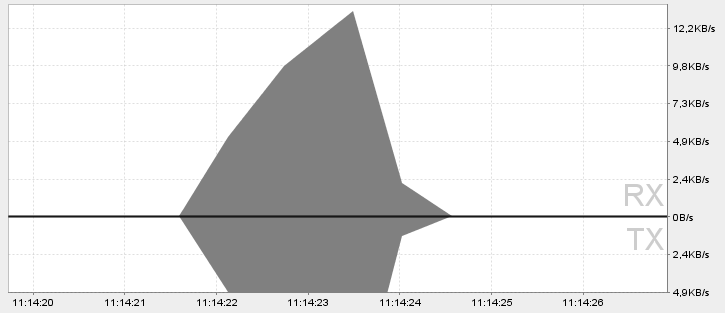
\includegraphics[width=0.45\textwidth]{figures/get_retrofit.png}} \qquad
	\subfloat[GET Request Jersey]{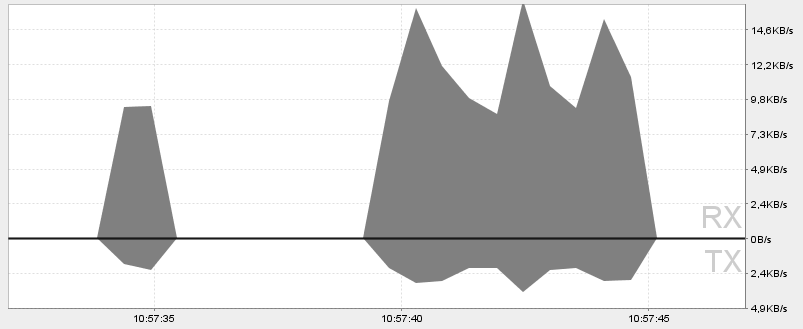
\includegraphics[width=0.45\textwidth]{figures/get_jersey.png}} \qquad
	\subfloat[GET Request Spring for Android]{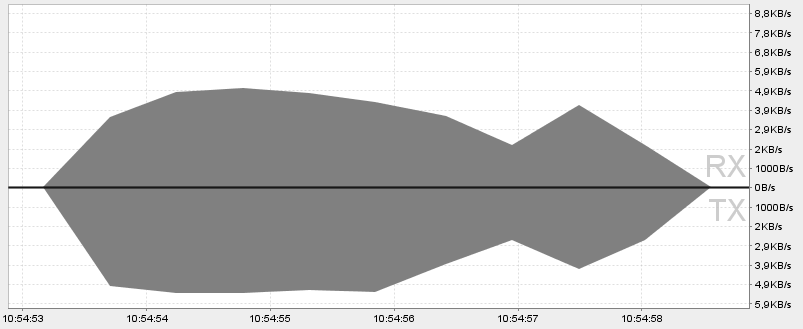
\includegraphics[width=0.45\textwidth]{figures/get_spring.png}} \qquad
	\subfloat[GET Request AndroidAnnotations]{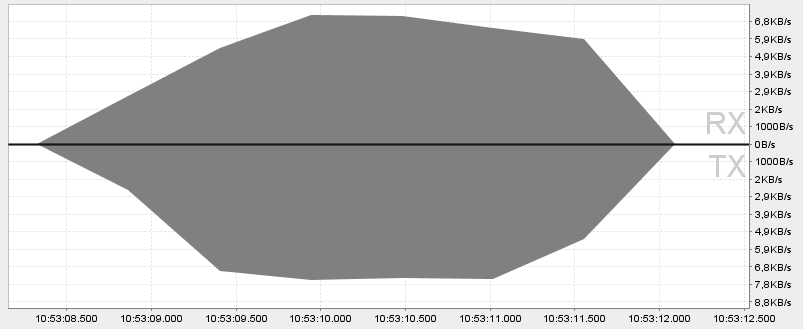
\includegraphics[width=0.45\textwidth]{figures/get_aa.png}}
	\caption{Zeitmessung der GET Requests} 
	\label{getRequests}
\end{figure} 

\newpage
Die Messung der Zeitdauer für einen POST Request ist aus der Abbildung \ref{postRequests} zu entnehmen. Dabei wurde die Zeit gemessen bis neu eingegeben Daten, um ein Kraftwerk anzulegen erfolgreich zum Server übermittelt wurden. Es konnte dabei festgestellt werden, dass alle Frameworks circa gleich lange benötigen, um die Daten zu übertragen. Spring for Android ist dabei minimal langsamer als die anderen, dies ist aber zu vernachlässigen, da diese Verzögerung keine Auswirkung auf die Usability für einen User hat \cite{meyer:performance}.

\begin{figure} [ht]
	\centering
	\subfloat[POST Request Retrofit]{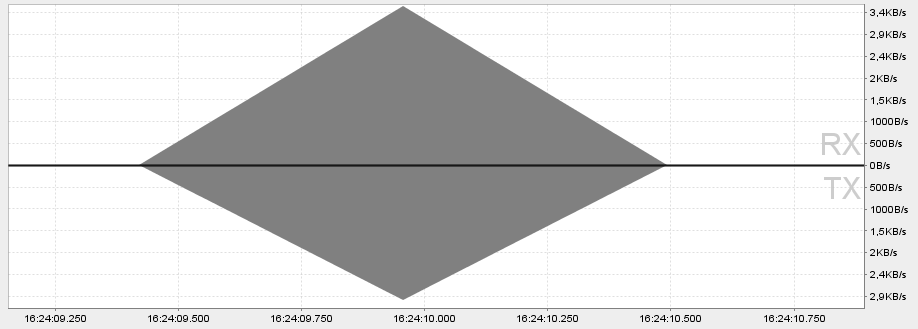
\includegraphics[width=0.45\textwidth]{figures/post_retrofit.png}} \qquad
	\subfloat[POST Request Jersey]{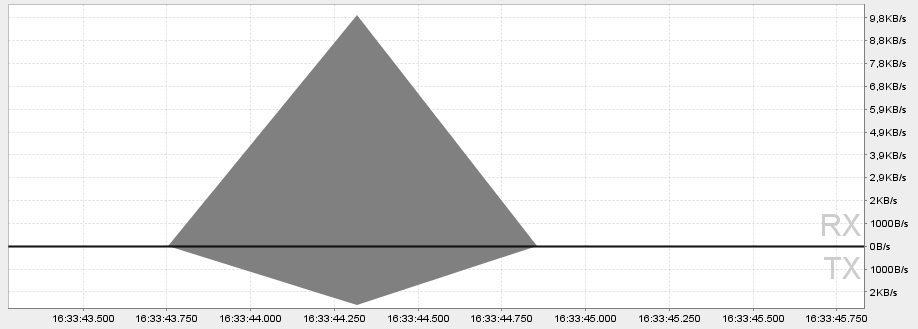
\includegraphics[width=0.45\textwidth]{figures/post_jersey.png}} \qquad
	\subfloat[POST Request Spring for Android]{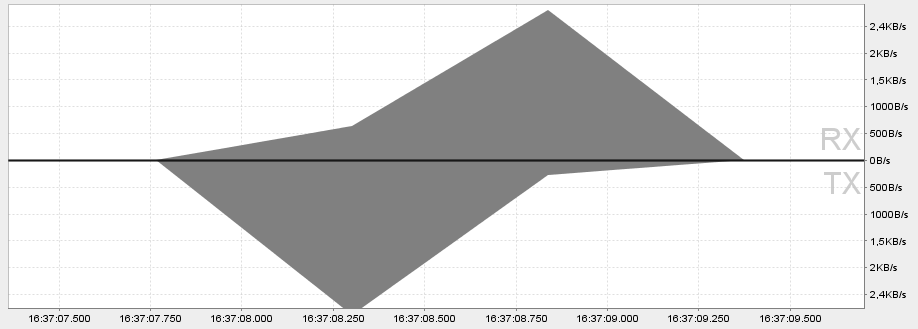
\includegraphics[width=0.45\textwidth]{figures/post_spring.png}} \qquad
	\subfloat[POST Request AndroidAnnotations]{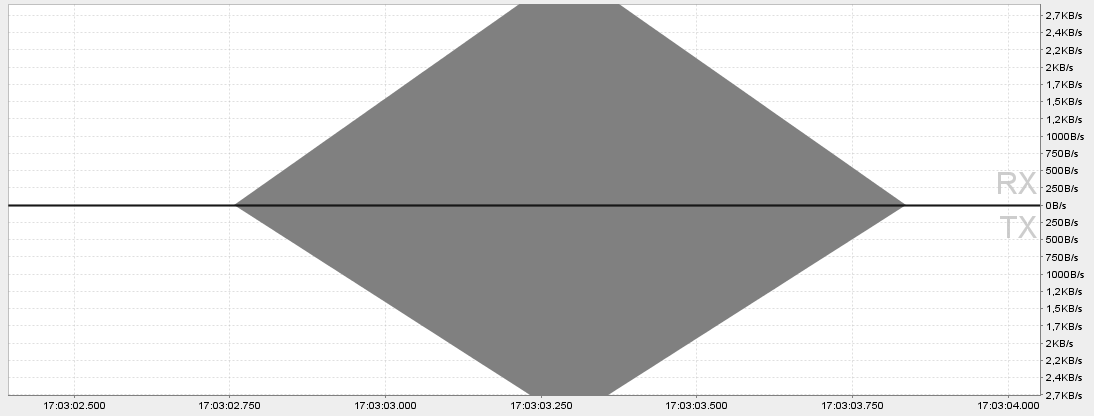
\includegraphics[width=0.45\textwidth]{figures/post_aa.png}}
	\caption{Zeitmessung der POST Requests} 
	\label{postRequests}
\end{figure} 

In der Abbildung \ref{cpuAuslastung} wird die CPU Auslastung der einzelnen Frameworks gegenübergestellt. Aus dieser Abbildung kann entnommen werden, das AndroidAnnotations die CPU am geringsten in Anspruch nimmt und Jersey am stärksten. Bei der Benutzung der Apps ist auch festzustellen, dass AndroidAnnotations und Retrofit am schnellsten arbeiten und eine flüssige Bedienung der Anwendung möglich ist. Jersey ist des öfteren langsam und hat kleinere Ruckler währende der Bedienung. Die Messungen konnten dabei den subjektiven Eindruck während der Bedienung der Apps bestätigen.

\begin{figure} [ht]
	\centering
	\subfloat[CPU Auslastung Retrofit]{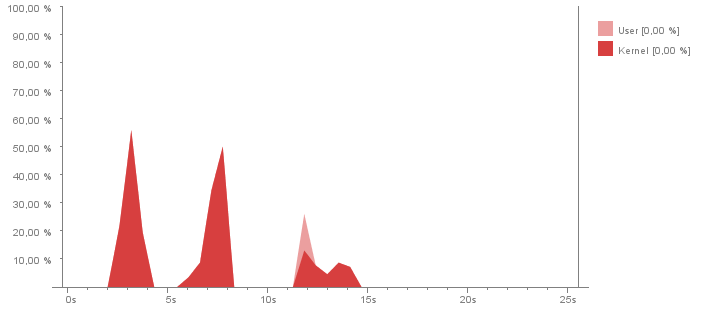
\includegraphics[width=0.45\textwidth]{figures/cpu_retrofit.png}} \qquad
	\subfloat[CPU Auslastung Jersey]{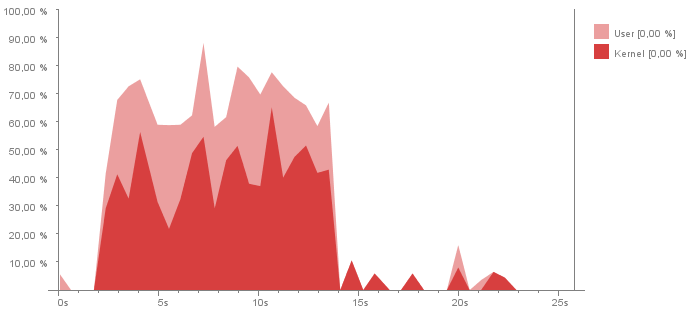
\includegraphics[width=0.45\textwidth]{figures/cpu_jersey.png}} \qquad
	\subfloat[CPU Auslastung Spring for Android]{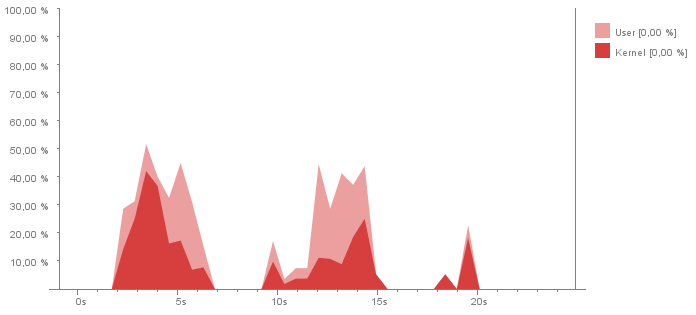
\includegraphics[width=0.45\textwidth]{figures/cpu_spring.png}} \qquad
	\subfloat[CPU Auslastung Request AndroidAnnotations]{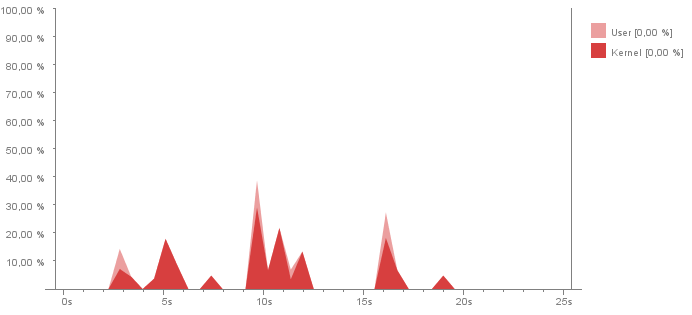
\includegraphics[width=0.45\textwidth]{figures/cpu_aa.png}}
	\caption{CPU Auslastung} 
	\label{cpuAuslastung}
\end{figure} 

{\large \textbf{Speicherplatz}}\\\\
Eine der größten Herausforderungen beim Implementieren von Apps ist der Hardwareunterschied der mobilen Geräte. Die Hardwarekomponenten unterscheiden sich nicht nur in der Displaygröße oder CPU Leistung, sondern auch im Speicherbereich \cite{joorabchi:challenges}. Sei es nun der zur Verfügung gestellte \acrfull{RAM} oder der interne Speicher, welcher bei manchen Geräten durch Speicherkarten erweitert werden kann. Je mehr und je größere Apps installiert werden, desto mehr leidet die Performance – insbesondere auf älteren oder Hardware schwächeren Geräten. Auch spielt die Installationszeit eine wichtige Rolle. User wollen Apps so schnell wie möglich nutzen, längere Installationszeiten sorgen schneller dafür, dass die Installation abgebrochen wird \cite{schaefers:apk}. Bei der Gegenüberstellung der APK Größe und der maximalen RAM Beanspruchung schnitt AndroidAnnotations am besten ab, Jersey am schlechtesten (siehe Tabelle \ref{tableVergleich}). 

\begin{figure} [ht]
	\centering
	\subfloat[benötigter RAM Retrofit]{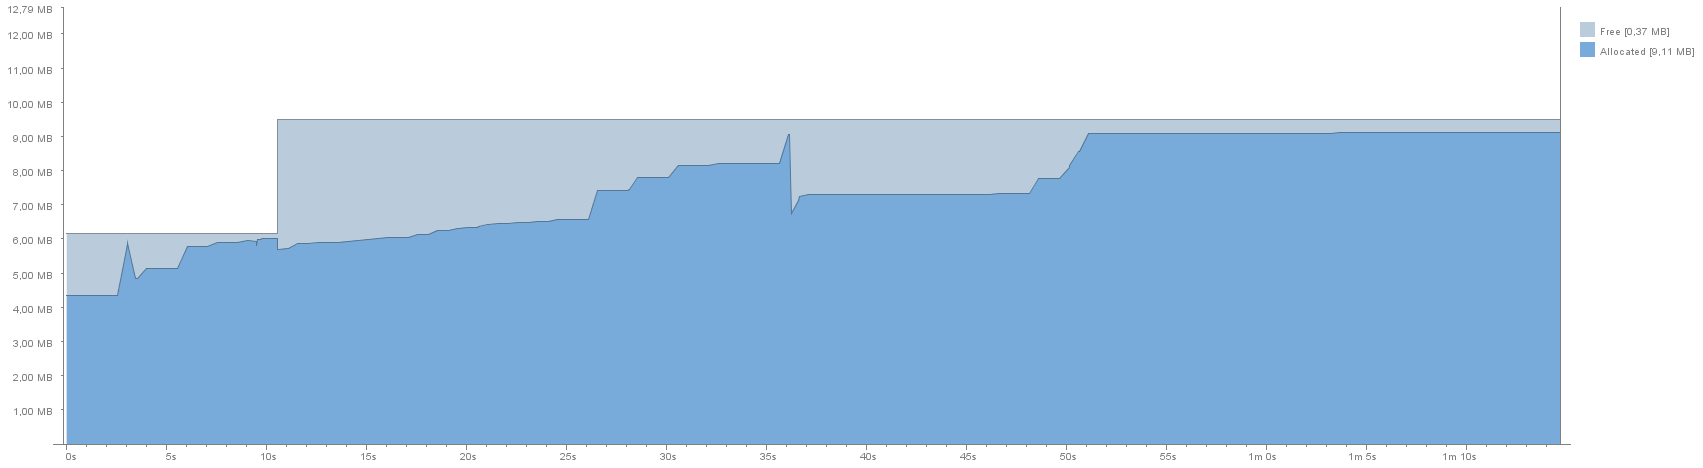
\includegraphics[width=0.48\textwidth]{figures/ram_retrofit.png}} \qquad
	\subfloat[benötigter RAM Jersey]{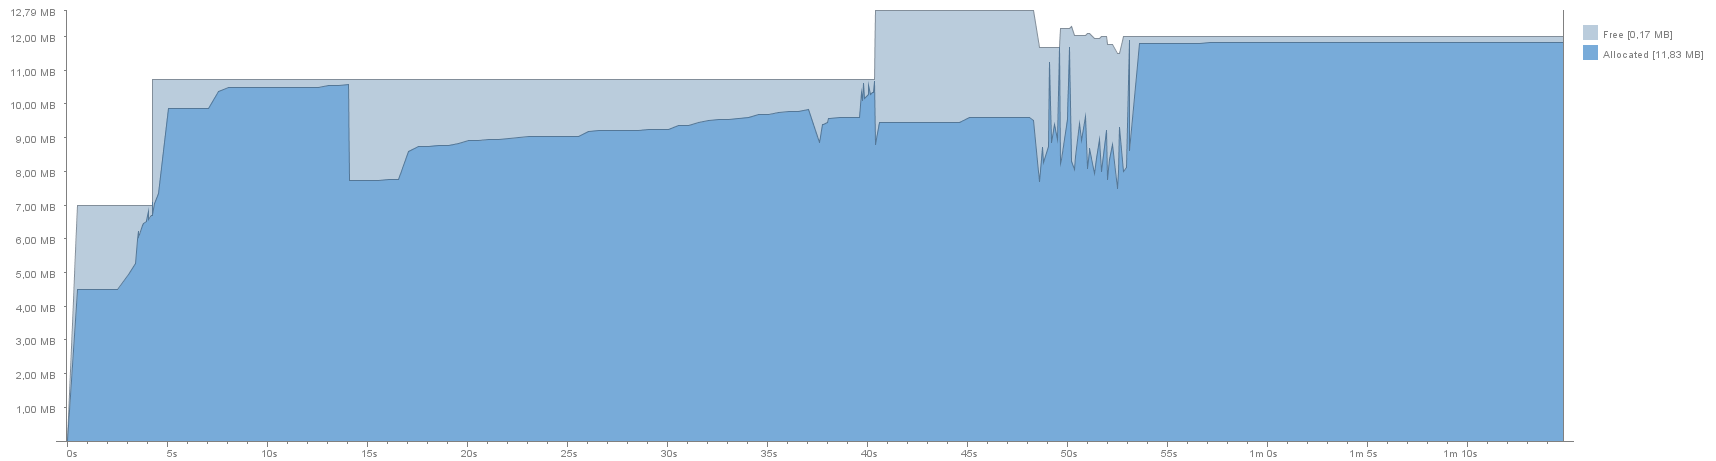
\includegraphics[width=0.45\textwidth]{figures/ram_jersey.png}} \qquad
	\subfloat[benötigter RAM Spring for Android]{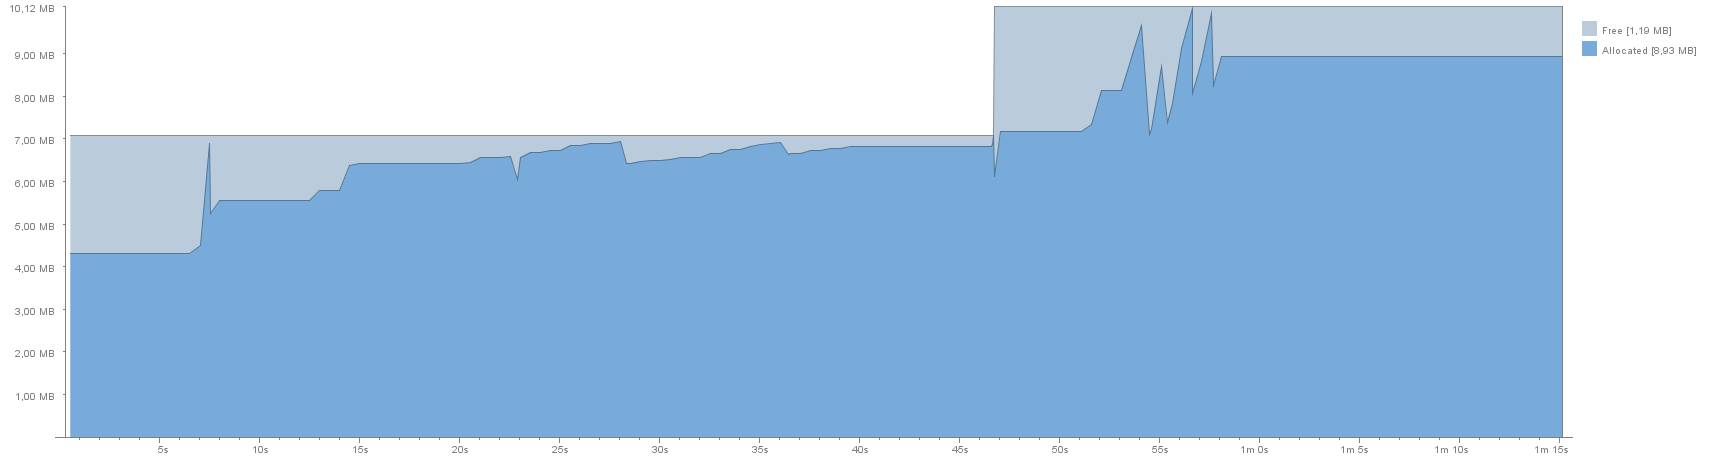
\includegraphics[width=0.45\textwidth]{figures/ram_spring.png}} \qquad
	\subfloat[benötigter RAM Request AndroidAnnotations]{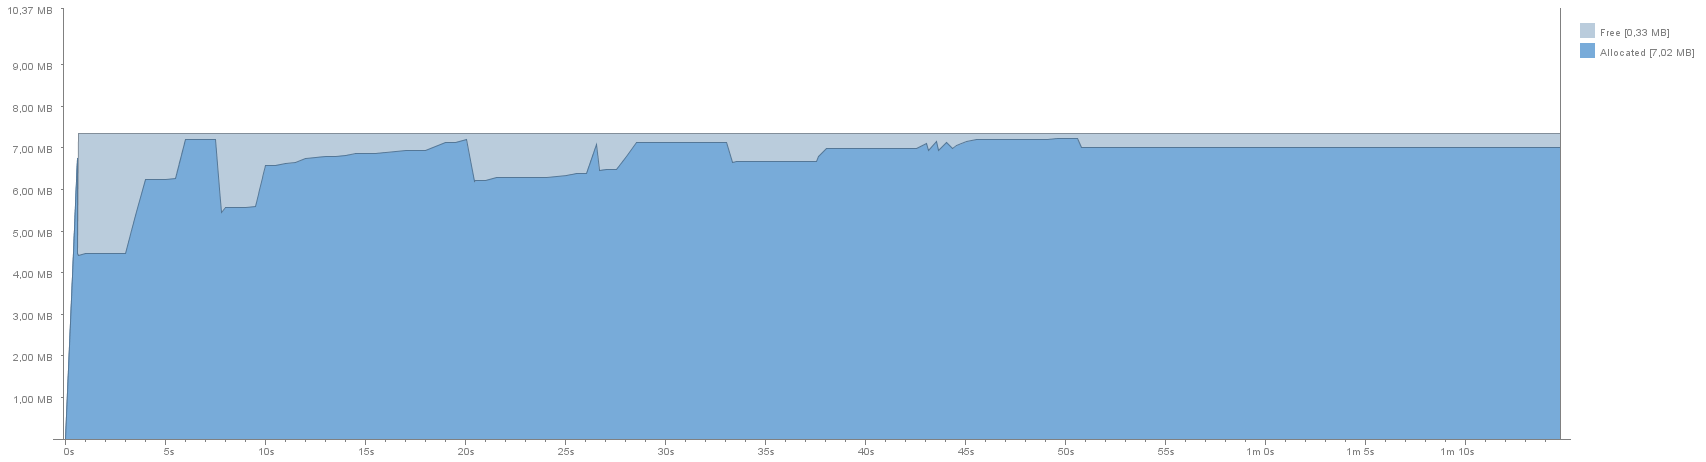
\includegraphics[width=0.45\textwidth]{figures/ram_aa.png}}
	\caption{benötigter RAM} 
	\label{ramB}
\end{figure} 

{\large \textbf{Erweiterte Technische Fähigkeiten der Frameworks}}\\\\
Sicherheit ist ein wesentliches Thema in der Informatik und auch für mobile Geräte. Denn die Apps sind nicht nur auf Informationen des Smartphones beschränkt, sondern haben auch Zugriff auf das Internet. OAuth ist ein Webstandard für den beschränkten Zugriff von Benutzer-Ressourcen auf Servern \cite{shehab:secure}. Dieser Standard wir von allen Frameworks unterstützt und ermöglicht einen sicheren und beschränkten Zugriff auf Ressourcen. 
\\\\
Alle evaluierten Frameworks unterstützten keine weiteren Übertragungsprotokolle außer HTTP. Die ACID-Eigenschaften werden auch von keinem der Frameworks implementiert. Soll aber ein Transaktionsmanagement clientseitig unterstützt werden, muss eine eigene Implementierung geschrieben werden. Dabei muss besonders darauf geachtet werden, dass alle Daten, die während einer Transaktion verwendet werden, gesperrt sind und sich nicht ändern dürfen, so lange bis die Transaktion Commited wird oder ein Rollback durchgeführt wird \cite{braun:Transaktionen}.
\\\\
Jersey hat eine serverseitige Referenzimplementierung. Für Spring for Android existiert ebenfalls eine Referenzimplementierung aus der Spring Familie. AndroidAnnoations hat keine direkt Referenzimplementierung, aber man kann auch auf jene der Spring Familie zurückgreifen - den die REST Implementierung von AndroidAnnoations basiert auf Spring for Android. Retrofit hat keine serverseitige Referenzimplementierung.
\\\\
AndroidAnnotations stellt als einziges Framework zusätzliche Dienste bereit, welche die Implementierung einer Android App erleichtern. Diese zusätzlichen Dienste sind unter anderem Dependency Injection oder Event Binding, siehe Kapitel \ref{androidannoations}.

\begin{landscape}
% m{3.5cm}|m{4.5cm}|m{4.5cm}|m{4.5cm}|m{4.5cm}
\renewcommand{\arraystretch}{1.3}
\begin{longtable}{m{3.5cm}|m{4.5cm}|m{4.5cm}|m{4.5cm}|m{4.5cm}}
	%	>{\centering \arraybackslash}m{3.5cm}|
	%	>{\centering \arraybackslash}m{4.5cm}|
	%	>{\centering \arraybackslash}m{4.5cm}|
	%	>{\centering \arraybackslash}m{4.5cm}|
	%	>{\centering \arraybackslash}m{4.5cm}}

      \caption{Gegenüberstellung der Frameworks} \\
	  \label{tableVergleich}	 
	  
	    & \textbf{Retrofit} & \textbf{Jersey} & \textbf{Spring for Android}  & \textbf{AndroidAnnotations}  \\ \hline
	    \textbf{\textit{Version}} & 
	    \textit{2.0} & \textit{2.0} & \textit{2.22.1} & \textit{4.0} \\ \hline \hhline{=====}
	   \multicolumn{5}{c}{\textbf{Entwicklungskultur}} \\ \hhline{=====}
	    
	  \textbf{Lizenz} &
	  Apache License Version 2.0 & CDDL Version 1.1 \newline GPL Version 2 & 
	  Apache License Version 2.0 & 
	  Apache License 2.0 \newline CDDL \\ \hline
	  \textbf{aktive Community} & Ja & Ja & Ja & Ja\\ \hline
	  \textbf{Dokumentation} & grundlegend & gut & gut  & gut \\ \hline 
		  \textbf{Codebeispiele} &  Ja  & nicht speziell für Android & Ja & Ja\\ \hhline{=====}
	  
	  \multicolumn{5}{c}{\textbf{Implementierung}} \\ \hhline{=====}
	  \textbf{Einbindung} & leicht & problematisch & leicht & leicht \\ \hline
	  \textbf{HTTP-Methoden} & GET, POST, PUT, DELETE, HEAD & GET, POST, PUT, DELETE, HEAD, OPTIONS  & GET, POST, PUT, DELETE, HEAD, OPTIONS & GET, POST, PUT, DELETE, HEAD, OPTIONS \\ \hline
	  \textbf{HTTP-Header} & erweiterbar & erweiterbar & erweiterbar & erweiterbar \\ \hline
	  \textbf{unterstützte\newline Medientypen} & alle möglichen, wenn Konverter für Typ vorhanden ist & alle möglichen, wenn Konverter für Typ vorhanden ist & alle möglichen, wenn Konverter für Typ vorhanden ist & alle möglichen, wenn Konverter für Typ vorhanden ist \\ \hline
	  \textbf{URL veränderbar} & Ja & Ja & Ja & Ja  \\ \hline
	  \textbf{asynchrone Requests} & Ja & Ja & Ja & Ja \\ \hline
	  \textbf{HATEOAS Konzept} & Nein & Ja & mithilfe von Spring HATEOAS & ohne Annotations und mithilfe von Spring HATEOAS \\ \hline 
	  \textbf{Error-Handling} & unterstützt & unterstützt & unterstützt & unterstützt \\ \hline
	
	   \newpage 
	    & \textbf{Retrofit} & \textbf{Jersey} & \textbf{Spring for Android}  & \textbf{AndroidAnnotations}  \\ \hhline{=====}
	  
	  \multicolumn{5}{c}{\textbf{Performance und Speicherplatz}} \\ \hhline{=====}
	  
	  \textbf{GET Request} & \textasciitilde3s & \textasciitilde12s  & \textasciitilde5s & \textasciitilde3.5s\\ \hline
	  
	  \textbf{POST Request} & \textasciitilde1s &  \textasciitilde1s & \textasciitilde1.5s & \textasciitilde1s \\ \hline
	  
	  \textbf{CPU Auslastung} & max. \textasciitilde55\%  & max. \textasciitilde87\% & max. \textasciitilde52\% & max. \textasciitilde40\%\\ \hline
	  \textbf{belegter RAM} & max. 9.11 MB & max. 11.83 MB & max. 8.93 MB & max 7.02 MB \\ \hline
	  \textbf{APK Größe} & 1.70 MB & 2.58 MB & 1.69 MB & 1.44 MB \\ \hhline{=====}

	   \multicolumn{5}{c}{\textbf{Erweiterte Technische Fähigkeiten}} \\ \hhline{=====}
	   
	   \textbf{Sicherheit} & OAuth2, SSL via OkHttp & OAuth2, SSL & OAuth2, SSL & OAuth2, SSL \\ \hline
	   \textbf{andere Protokolle außer HTTP} &  Nein & Nein & Nein & Nein\\ \hline	   
	   \textbf{ACID-Eigenschaften} & Nein & Nein & Nein & Nein \\ \hline
	   \textbf{Server Implementierung} & Nein & Ja &  Spring Framework & Nein (eventuell Spring Framework) \\ \hline
	   \textbf{zusätzliche Dienste} & Nein & Nein & Nein & Ja \\ \hline
 
\end{longtable}
\end{landscape}

\section{Evaluierung im Kontext Revex2020}
Als REST Frameworks sind sowohl Retrofit, Spring for Android und AndroidAnnoations geeignet. Von Jersey als REST Framework ist abzuraten, da dieses Framework nur mithilfe eines Workarounds benützt werden kann. Darüber hinaus schneidet Jersey im Performance- und Speichervergleich am schlechtesten ab.
\\\\
Vergleicht man nun jene anderen drei ist der Unterschied minimal. Retrofit weißt eine etwas schwächere Dokumentation auf, da gerade eine neue Version erschienen ist und die Dokumentation teilweise noch nicht an die neueste Version angepasst wurde (Stand Ende 2015). Spring for Android ist im Lesezugriff langsamer, was einen minimalen Nachteil darstellt - da das Anzeigen einer großen Datenmenge länger dauert. Retrofit und AndroidAnnoations haben einen leicht zu lesenden Code, da dieser Annotations basiert ist. Dadurch verringert sich der zu schreibende und wartende Code, wodurch die Entwicklung beschleunigt und die Wartbarkeit verbessert werden kann \cite{cleanCode}.
\\\\
Zusammenfassend ist zu empfehlen AndroidAnnoations als REST Framework zu verwenden. Dieses Framework arbeitet Ressourcenschonend und unterstützt alle nötigen Anforderungen, welche für das Revex Projekt benötigt werden. Der HTTP-Header kann erweitert und verwendet werden und es werden alle benötigten HTTP-Methoden (GET, PUT, POST und DELETE) unterstützt. Des weiteren sind sowohl asynchrone Requests und das behandeln von Fehlern möglich. Ein weiterer Pluspunkt von AndroidAnnoations sind die zusätzlicher Dienste, welche die Implementierung einer Android App erleichtern. Sollen diese Dienste, welche in AndroidAnnoations enthalten sind, mit den anderen Frameworks verwendet werden, müssen zusätzliche Drittanbieter Bibliotheken hinzugefügt werden. Dadurch wird, aber der benötigte Speicherplatz der App erhöht.

\section{Persönliches Fazit zu den Frameworks}
Es folgt nun ein kurzer persönlicher Eindruck zu den Frameworks. Wo sind Probleme während der Implementierung aufgetreten und welche Aspekte besonders positiv aufgefallen sind.
\\\\
{\large \textbf{Retrofit}}\\\\
Retrofit ist ein Annotations basiertes Framework, wodurch der Code leicht verständlich und kurz zu schreiben ist. Das Einbinden in ein Projekt gestaltet sich als sehr einfach, es müssen nur die nötigen Abhängigkeiten in die gradle-Datei des Projektes eingefügt werden. Problematisch bei der Implementierung war die teilweise veraltete Dokumentation. Es konnte anfangs nicht festgestellt werden, auf welche Version des Frameworks die gefundene Beschreibung Bezug nahm. Bei mehrmaligem Zugriff auf die offizielle Dokumentation konnte aber festgestellt werden, dass diese laufend erweitert und auf die neueste Version abgeändert wurde. Dies weißt auf eine aktive Community hin. Performance technisch konnten keinerlei Probleme festgestellt werden, das Framework arbeitet flüssig und es kam zu keinen Verzögerungen während der Nutzung der App.
\newpage
{\large \textbf{Jersey}}\\\\
Jersey war am problematischsten zu implementieren, da es am längsten gedauert hat dieses Framework unter Android verwenden zu können. Es musste eine umfangreiche Recherche im Internet durchgeführt werden, bis die Probleme dieses Frameworks mit Android festgestellt werden konnten. Danach musste noch einige Zeit investiert werden, bis ein funktionierender Workaround für die Probleme gefunden werden konnte. Die clientseitige Dokumentation des Framework ist gut und liefert alle relevanten Informationen für den Implementierungsprozess. Während der Nutzung der App kam es immer wieder zu Verzögerungen, bis alle relevanten Daten geladen wurden. Dies hat wesentlich Auswirkungen auf die Usability, da eine längere Wartezeit nötig ist, bis dem User alle Daten angezeigt werden. Jersey schnitt im Performance- und Speichervergleich am schlechtesten ab. Es ist daher deutlich festzustellen, dass die clientseitige Implementierung von Jersey nicht für Android optimiert wurde.
\\\\
{\large \textbf{Spring for Android}}\\\\
Das Einbinden von Spring for Android in ein Projekt gestaltet sich als trivial, es müssen nur die nötigen Abhängigkeiten in die gradle-Datei des Projektes eingefügt werden. Es sind sowohl eine gute Dokumentation, als auch Beispielcodes auf der offiziellen Homepage verfügbar. Der Code ist gut strukturiert, aber nicht so leicht verständlich, wie bei Annotations basiertes REST Frameworks. Daher musste mehr Zeit in das Implementieren der REST Schnittstellen investiert werden, da auch mehr Code zu schreiben war.  Performancetechnisch lag dieses Framework im Mittelfeld, großteils arbeitet es sehr flüssig. Nur beim Abrufen großer Datenmengen kommt es zeitweise zu einer minimalen Verzögerung.
\\\\
{\large \textbf{AndroidAnnotations}}\\\\
Das Einbinden und Verwenden von AndroidAnnotations ist sehr einfach, es sind wiederum nur alle nötigen Abhängigkeiten in die gradle-Datei des Projektes einzufügen. Die Dokumentation und gefunden Code Beispiele sind ebenfalls sehr gut und enthalten alle benötigten Informationen für die Implementierung. Da AndroidAnnotations ein Annotations basiertes Framework ist, ist der Code gut lesbar und schnell zu schreiben, was den Implementierungsprozess erheblich verkürzt. Performance technisch schnitt dieses Framework am besten ab, es arbeitet flüssig und es kam zu keinerlei Verzögerungen während der Nutzung. Ein großer Mehrwert dieses Framework ist, das zur Verfügung stellen zusätzlicher Dienste, fernab der REST Kommunikation. Dadurch gestaltet sich das Implementieren einer Android App als einfacher. Da auch Annotation für andere Bereiche existieren, wird der zu schreiben Code für eine App stark reduziert. Zum Beispiel existiert Annotationen für das behandeln von Events bei Views, es werden keine anonymen Listener Klassen mehr benötigt.